% TODO: Proof read paper and make it nicer with some 
% paragraphs and LaTeX typesetting.
% TODO: Reference every figures atleast once in text.
\documentclass[sigconf]{acmart}
\usepackage{booktabs}
\usepackage{diagbox}

\AtBeginDocument{
  \providecommand\BibTeX{{
      \normalfont B\kern-0.5em{\scshape i\kern-0.25em b}\kern-0.8em\TeX}}}

\settopmatter{printacmref=false}
\renewcommand\footnotetextcopyrightpermission[1]{}

% Custom Operator
\newcommand{\Var}{\operatorname{Var}}

% Our Algorithm Engineering Conference
\acmConference[AEPRO 2023]{AEPRO 2023: Algorithm Engineering Projects}{Jena, Germany}

\begin{document}

\title[Bildqualitätsverbesserung für Bilder von Dokumenten]
{Bildqualitätsverbesserung für Bilder von Dokumenten \\\large
  Algorithm Engineering 2023 Projekt Paper}

\author{Mario Baars} \affiliation{
  \institution{Friedrich Schiller University Jena} \country{Germany}}
\email{mario.louis.baars@uni-jena.de}

\author{Eric Günl} \affiliation{
  \institution{Friedrich Schiller University Jena} \country{Germany}}
\email{eric.günl@uni-jena.de}

% TODO: Finetune Abstract
\begin{abstract}
  In diesem Paper wird über die Konzeption, Entwicklung und
  Optimierung eines Bildqualitätsverbesserungsprogramm berichtet. Es
  werden die verwendeten Algorithmen, die Prototypisierung in
  \texttt{Python}, bis hin zu einer optimierten, parallelisierten
  Version des Programms in \texttt{C++} beleuchtet. Darüber hinaus
  werden Performanz, Grad der Effektivität und die Design
  Entscheidungen des Programms diskutiert.
  
  Entstanden ist hierbei ein plattform-übergreifendes Programm,
  welches system- und kompilier-agnostisch schlechte Bilder von Dokumenten
  in eine gut druckbare Form überführt. Durch die Portabilität und
  gute Performanz, kann dieses Programm effektiv in der Kommandozeile
  für die Bildqualitätsverbesserung verwendet werden. Darüber hinaus
  ermöglicht das Bereitstellen von zwei Parameter als
  Kommandozeilenoption, den Nutzer ad-hoc ideale Parameter für das
  zuverbesserende Bild zufinden, ohne das Programm erneut kompilieren
  zu müssen.
\end{abstract}

\keywords{Image Enhancement, Programm Optimization, Portability}

\maketitle

\let\thefootnote\relax\footnotetext{AEPRO 2023, \today, Jena,
Germany. Copyright \copyright 2023 for this paper by its
authors. Use permitted under Creative Commons License Attribution
4.0 International (CC BY 4.0).}

\section{Ziel des Projekts}
Das Projekt Bildverbesserung für aufgenommene Dokumente hat das Ziel
ein Foto von einem schriftlichen Dokument, welches im \texttt{ppm} P$3$
Format vorliegt, so zu verbessern, dass Schrift und Hintergrund in
einem hohen Kontrast zueinander stehen. Dabei ist die best mögliche
Verbesserung, dass für jeden Pixel entschieden wird, ob er zur Schrift
oder zum Hintergrund gehört, wie das bei einem Dokument in einem
Texteditor der Fall wäre. Wir haben uns dazu entschieden tatsächlich
für jeden Pixel zu entscheiden ob er zur Schrift oder zum Hintergrund
gehört und keine Grauwertabstufungen in unserem Ausgabebild (auch im
\texttt{ppm} P$3$ Format) zu erlauben. Dies ist durch Bildrauschen,
Helligkeitsgradienten, oder Defokussierung eine herausfordernde
Aufgabe die wahrscheinlich meist keine $100$\%ige Trefferquote für jeden
Pixel haben wird. Dennoch versuchen wir mit unserem Programm so nah
wie möglich an dieses Ziel heranzukommen.

\section{Programm}
Das komplette Programm wurde in \texttt{Python} entwickelt. Die hier
aufgezählten Filter und viele weitere, die nicht effizient oder
wirksam waren, wurden in \texttt{Python} implementiert und
getestet. Danach wurde das Programm in \texttt{C++} übersetzt. Nachdem
es mit allen Funktionen in \texttt{C++} implementiert war, wurde das
Programm optimiert.

Das Programm lässt sich in grob in $4$ Bereiche unterteilen.

\subsection{Einlesen des Bildes}
Die \texttt{ppm} Datei wird in einen Buffer geladen. Danach werden
einzeln das Dateiformat, die Dimensionen und der Maximale Wert
eingelesen.  Danach wird der Buffer Pixel für Pixel durchlaufen und
aus den RGB Werten ein Grauwert errechnet. Dies geschieht mit den
Color conversion Werten von \emph{OpenCV}. Die errechneten Werten werden in
einem $2$D Array gespeichert.

\subsection{Algorithmen}
\subsubsection{Moving Normalization Filter}
Dieser Filter bewirkt, dass dunkle und helle Gebiete im Bild
aneinander angeglichen werden. Ein möglicher Helligkeitsgradient der
über das gesamte Bild verläuft wird mit diesem Filter geglättet, was 
in der Abbildung~\ref{fig:effect_moving_norm} zusehen ist. Der obere Graph zeigt mögliche
Originaldaten, bei welchen der Wert über den gesamten Bereich
sinkt. Die $2$ Kerben bei $20$ und $60$ zeigen hier die geringeren
Werte (wo im Bild die schwarze Schrift wäre) an, die detektiert werden
sollen. Mit einem festen Schwellwert ist dies nicht möglich. Deshalb
teilt man jeden einzelnen Wert durch den Mittelwert seiner
Umgebungswerte. Dies normalisiert den Hintergrund auf den Wert $1$
ohne dabei örtliche Gradienten wie die Schrift auszulöschen. Der
untere Graph zeigt, dass die Kerben immer noch deutlich detektierbar
sind und der Hintergrund einen festen Wert angenommen hat. Um die
Kerben herum ist der Wert sogar etwas höher als der Hintergrundwert,
was zusätzlich nützlich ist um Schrift von Hintergrund zu separieren~\cite{guenl2021}.

\begin{figure*}[htbp]
  \centering
  \includegraphics[width=0.7\linewidth]{./graphics/effect_moving_norm.png}
  \caption{Die Datenverteilung bevor (oben) und nach (unten) der
    Anwendung des \emph{Moving Normalization Filter}.}
  \label{fig:effect_moving_norm}
\end{figure*}

\subsubsection{Adaptiver Schwellwert Filter}
Der Schwellwert um zu entscheiden, ob der Pixel Hintergrund oder
Schrift ist, wird in unserem Algorithmus adaptiv anhand von $2$
lokalen Variablen und $3$ Parametern errechnet. Dazu wird das Array in
Bereiche aufgeteilt. Von diesen Bereichen wird die Varianz des schon
gefilterten Bildes berechnet. Dies ist die erste Variable der
Schwellwertformel. Für die zweite Variable wird aus dem original Bild
ein Histogramm linearisiertes Bild erzeugt.  Dies ist notwendig, da
besonders dunkle und auch sehr helle Bilder einen ähnlichen
Wertebereich haben müssen, damit die Schwellwertformel für alle Bilder
funktioniert. Das Histogramm linearisierte Bild wird in die selben
Bereiche unterteilt und für jeden Bereich wird der maximale Wert
ermittelt. Dies ist die zweite Variable der Formel.  Die Formel
lautet:
\begin{equation}
  S = m \cdot \Var + n + \sqrt{b_{\max}} \cdot f
\end{equation}
$\Var$ ist die Varianz. $b_{\max}$ ist der maximale wert des
linearisierten Bildes.  Die Parameter sind:

\begin{itemize}
\item $m$: Faktor (Gewicht) für die Varianz
\item $n$: Summand um die zu justieren
\item $f$: Faktor für die Wurzel aus der maximalen Helligkeit
\end{itemize}

Diese Formel ist durch umfangreiches Testen von Variablen, die einen Einfluss
auf den Schwellwert haben entstanden. Die Parameter wurden so
ausgewählt, dass für die Beispielbilder das bestmögliche Ergebnis nach
unserer visuellen Beurteilung herauskam.  Sowohl der Parameter $n$ als
auch $m$ sind bei Aufruf des Programms einstellbar, um den Schwellwert
für das jeweilige Bild anzupassen. Dabei sollte der Wert $n$ zwischen
$0.2$ und $0.9$ liegen. Falls des Verbesserte Bild zu viele dunkle
Stellen aufweist sollte der $n$ Wert gesenkt werden. Wenn jedoch teile
der Schrift nicht erkannt werden und als Hintergrund detektiert werden
muss der $n$ Wert erhöht werden. Selbiges gilt für den $m$ Wert.  Hier
liegt der Bereich zwischen $0.2$ und $0.6$.

Im Programm wurde kein Filter zur Rauschunterdrückung implementiert,
da nach einigen Test mit zum Beispiel einem adaptiven
Mittelwertfilter, welcher die globale und lokale Varianz des Bildes
berücksichtigt, festgestellt wurde, dass keine signifikante
Verbesserung des Bildes aufgetreten ist. Die meisten Bilder von
Dokumenten sind nicht in einem Maß verrauscht, sodass Schrift nicht
vom Hintergrund unterscheidbar wäre~\cite{denzler2021}.


\subsection{Erstellen einer Ausgabe \texttt{ppm} Datei}
Erstellen einer Ausgabe \texttt{ppm} Datei Das erzeugte boolesche
Array mit nur Einsen und Nullen wird Stück für Stück mittels eines
Buffers der Größe $80$KBit in eine \texttt{ppm} P3 Datei geschrieben.

\begin{figure*}[htbp]
  \centering
  \includegraphics[width=\linewidth]{./graphics/comparison.png}
  \caption{Vergleich zwischen dem bereitgestellten Bild (links) und
    dem durch das Programm verbesserte Bild (rechts). Die verwendeten
    Parameter des \emph{Adaptive Thresholds} für die Verbesserung
    waren $m = 0.5$ und $n = 0.84$.}
  \label{fig:comparison}
\end{figure*}

\subsection{Optimierung}
Mit Zeitmessungen der einzelnen Bereiche konnte für $3$ Versionen des
Programms die Laufzeiten verglichen werden.  Dabei wurden das Programm
in Python, das nicht optimierte Programm in \texttt{C++} und das optimierte
Programm in \texttt{C++} verglichen: Als Bild wurde dabei eine ppm P$3$ Datei mit
$18.4$ MB verwendet. Die Laufzeitmessungen wurden auf dem selben PC, welcher $4$ Kerne besitzt, durchgeführt.

\begin{table}[htbp]
  \caption{Performance zwischen den unterschieldichen Iterationen des
    Bilderverbesserungsprogramms in Millisekunden.}
  \label{tab:vergleich_optimierung}
  \begin{tabular}{|l|l|l|l|}
    \hline
    \diagbox{Funktion}{Stadium} & \texttt{Python} & \texttt{C++} & \texttt{C++} optimiert \\
    % Funktion & & & \\
    \hline
    Laden des Bildes             & $910$ & $471$ & $116$ \\
    Moving Norm Filter           & $69500$ & $5118$ & $1203$ \\
    Adaptiver Schwellwert Filter & $2270$ & $277$ & $295$ \\
    Speichern des Bilds          & $680$ & $474$ & $210$ \\
    \hline
    Gesamtes Programm            & $73360$ & $6341$ & $1825$ \\
    \hline
\end{tabular}
\end{table}

Wie in der Tabelle~\ref{tab:vergleich_optimierung}zu sehen ist verbessert sich die Performance des
Python Programms zum \texttt{C++} Programm um mehr als das $10$-fache.  Auch die
Optimierung des \texttt{C++} codes bringt eine Performance Steigerung von $250$\%.

\subsubsection{Beschleunigung des Ladevorgangs der ppm Datei in ein Array}
 In der nicht optimierten Variante des \texttt{C++} Programms wird jeder Wert einzeln
aus der ppm Datei in eine Pixel Struktur geschrieben, welche in ein $2$D
Array gespeichert wird. Danach wird dieses Array durchlaufen und für
jeden RGB Wert der Grauwert berechnet und in ein neues Array
geschrieben.  Die optimierte Version lädt die gesamte ppm Datei in
einen Buffer. Dieser Buffer wird dann Char für Char durchlaufen und
die RGB Werte in Grauwerte umgerechnet und in ein Array
gespeichert. Dies bringt eine performance Steigerung von $300$\%.

\subsubsection{Parallelisierung des Moving Norm Filters}
Um diese Funktion zu optimieren wurden $2$ mal $2$ for Schleifen mit \texttt{omp for collapse(2)
schedule(static)} parallelisiert. Je nach Anzahl der Kerne des PCs
kann dies zu unterschiedlichen Performance Steigerungen führen. Die
Optimierung dieser Funktion ist am wichtigsten, da Sie auch der
Bottleneck des Programms ist.

\subsubsection{Beschleunigung des Speicherns der resultierenden Bild Datei}
Auch bei dieser Funktion werden die Daten zur Optimierung der Performance in
einen Buffer geschrieben, welcher dann in die Datei geschrieben wird.
Dies bringt eine Verbesserung im Vergleich zur Variante des Wert für
Wert in die Datei schreiben um $100$\%.

% TODO: newline
Zudem können die Flags \texttt{-Ofast} und \texttt{-ffast-math} genutzt werden um das
schon optimierte Programm zu Verbessern. Mit diesen beiden Flags
erhält man eine Laufzeit des kompletten Programms von $422$ ms und damit eine weitere
Performanzsteigerung von $300$\%.

\subsection{Tests}
Die Natur des Programms deutet eher auf die Verwendung von Systemtests
statt Unit-Tests oder Integrationtests. Das Kernstück der Programme sind die Algorithmen, 
die in den vorigen Abschnitten genauer beschrieben wurden. Diese Algorithmen sind 
so designed, dass sie bei einem gültigen Eingabebild im P$3$ \texttt{ppm}-Format auch gültige Zwischenergebnisse liefern.
Somit zeigt sich die bedeutungsvolle Gültigkeit der Funktionen erst durch die Anwendung aller Algorithmen
in einem integralen System. Deshalb wurde das Programm anhand von der Anwendung auf
verschieden beschaffene Eingabebilder getestet.

\subsection{CMake}
Für maximale Portabilität wurde \texttt{CMake} gewählt, um dessen
plattform-übergreifende Eigenschaften auszunutzen. Es gibt $2$
\texttt{CMakeLists.txt} Dateien in den die Instruktionen für das Bauen
des Programms zufinden sind. Beim Aufruf der \texttt{CMakeLists.txt}
in dem selben Ordner wie die \texttt{main.cpp} Datei wird die sekundäre
\texttt{CMakeLists.txt} Datei, die die \texttt{image\_enhancer\_lib} Bibliothek
baut, aufgerufen.  Die minimal Anforderungen dieses Programm zu
kompilieren sind ein \texttt{C}/\texttt{C++} Compiler, mit
\texttt{C++14}-Standard und die \texttt{CMake} Version $3.9$.

\section{Ergebnisse}
\begin{figure*}[htbp]
  \centering
  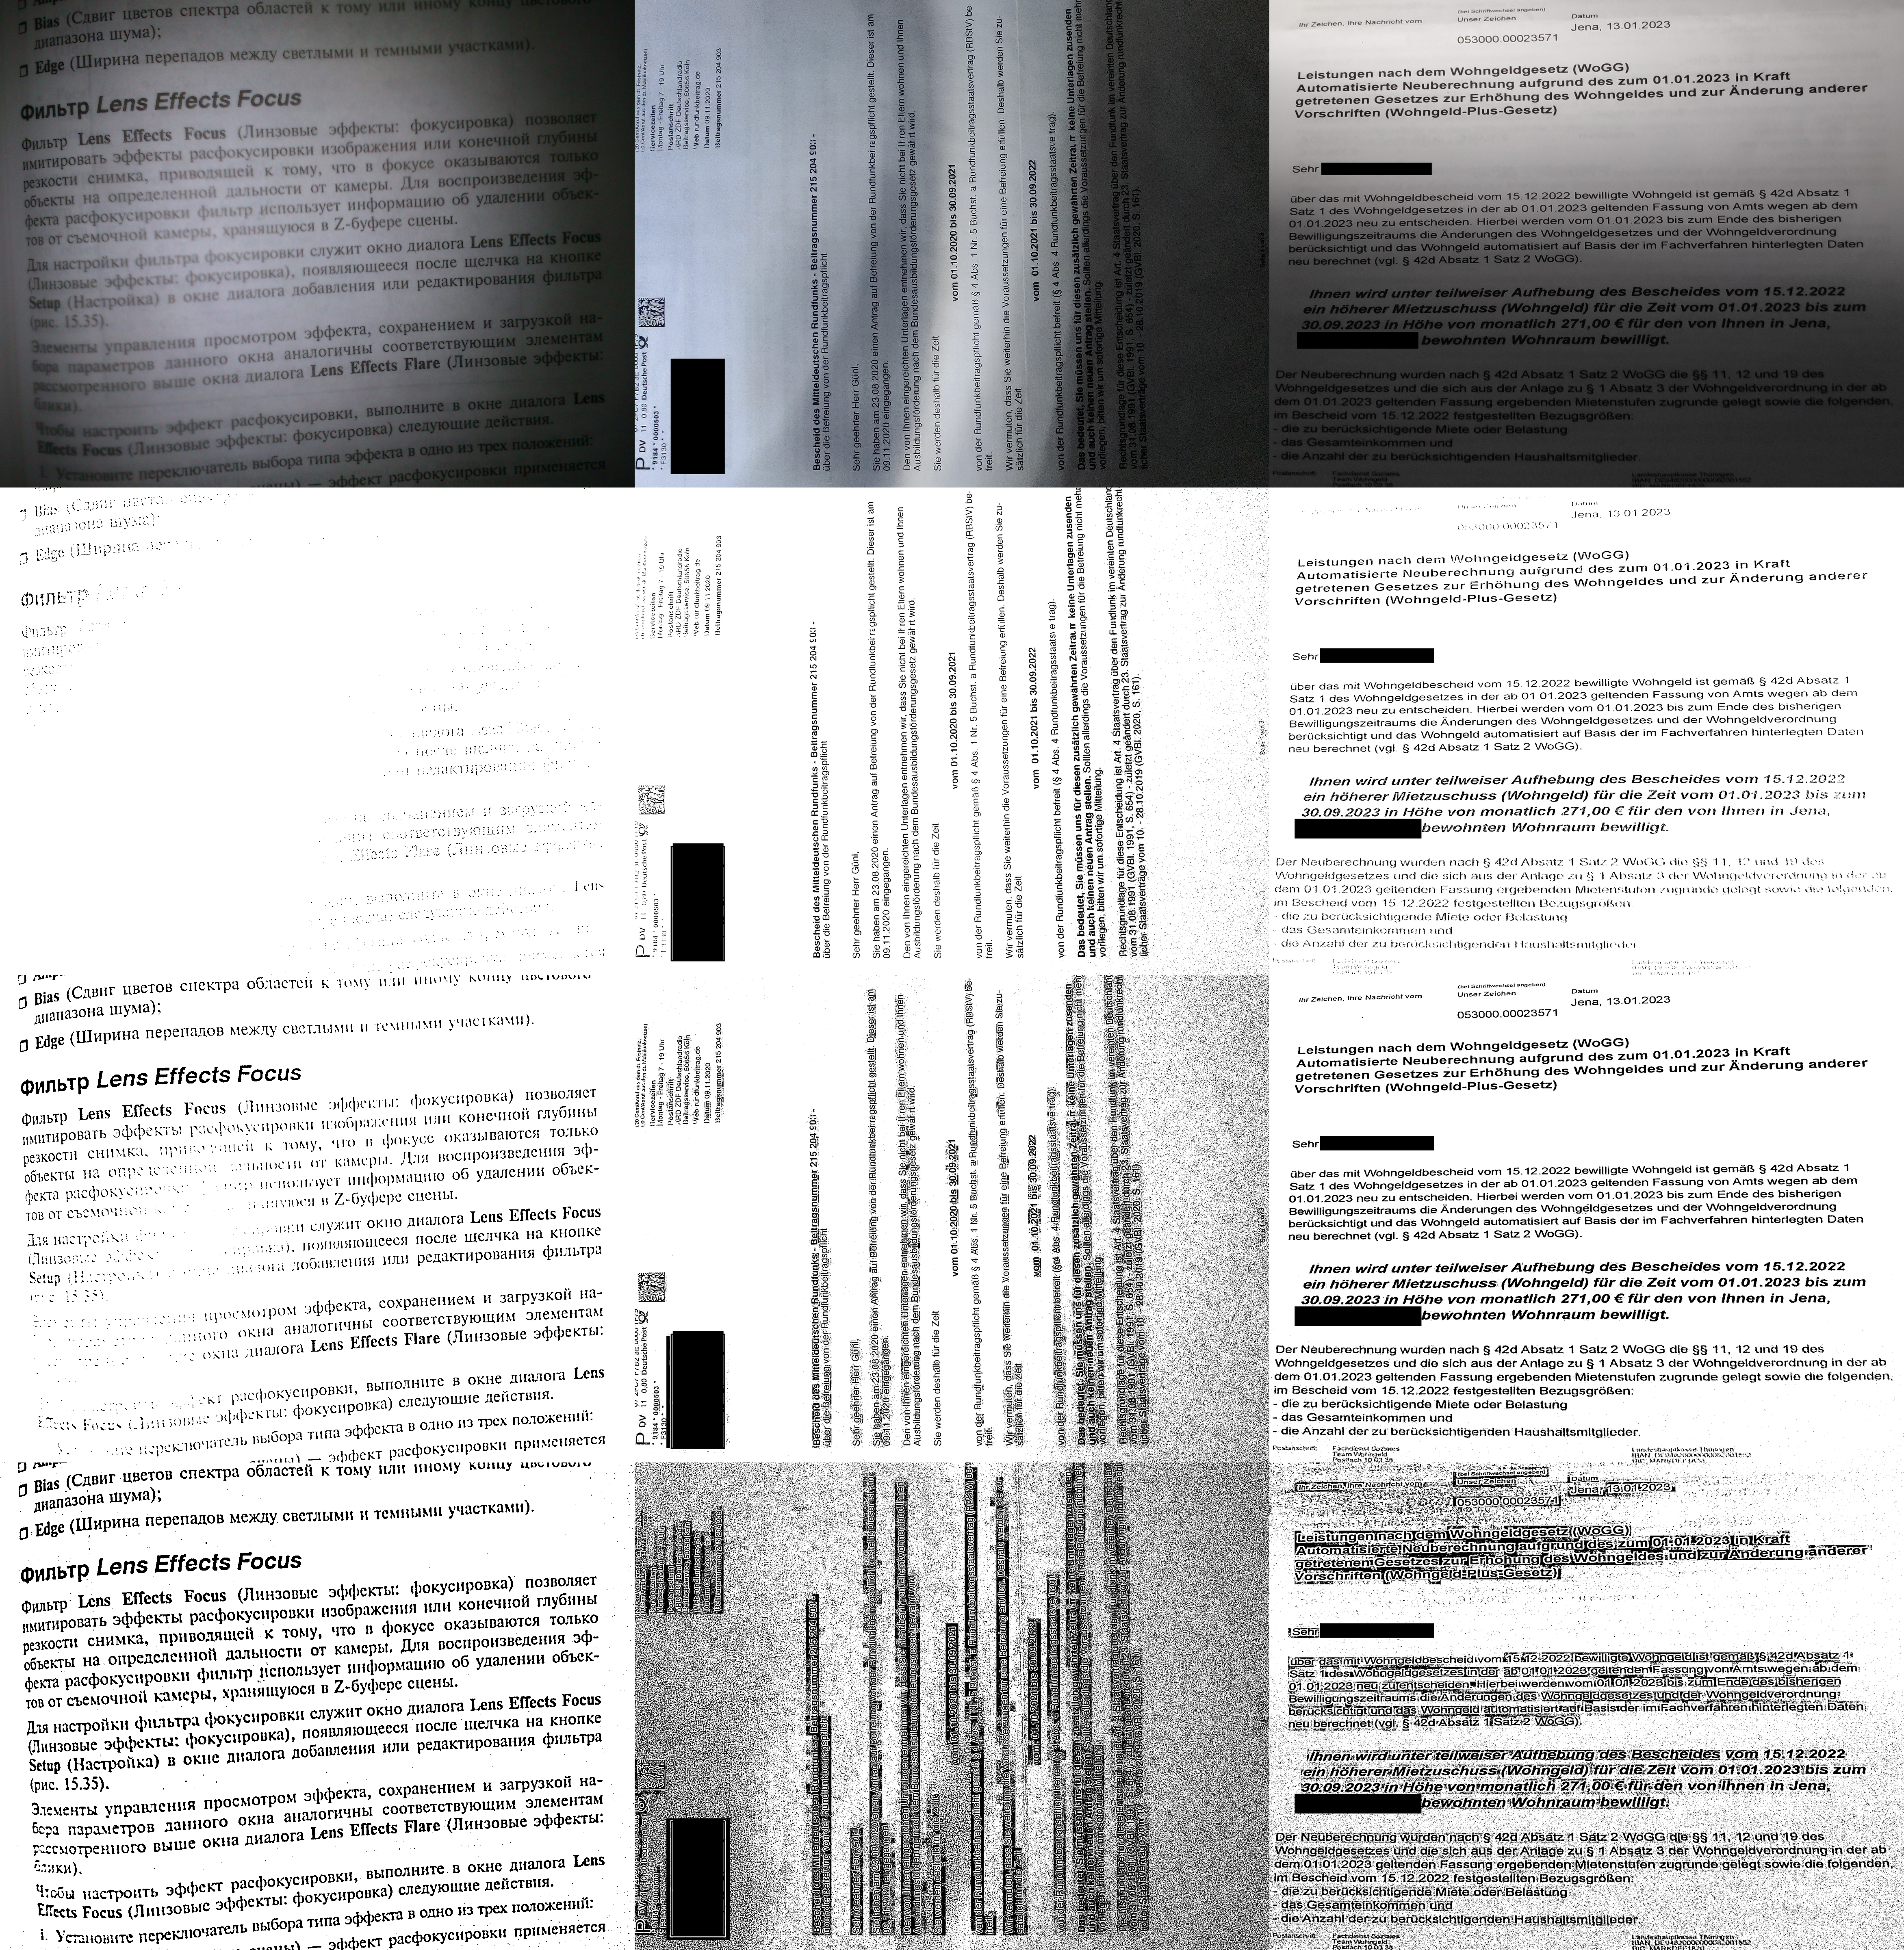
\includegraphics[width=\linewidth]{./graphics/image_matrix.png}
  \caption{Vergleich zwischen den Bildqualitätsverbesserung von unterschiedlichen
           Testbilder. Von oben nach unten: Original Bild, Verbesserter Bilder mit den
           Parameter: $m=0.3$, $n=0.3$; $m=0.45$, $n=0.7$; $m = 0.5$, $n = 0.84$.}
  \label{fig:image_matrix}
\end{figure*}

Wie in Abbildung~\ref{fig:image_matrix} zu sehen ist hängt die Qualität des Bildes stark
von den Parametern ab, die übergeben werden. Je dunkler das Bild,
desto geringer müssen die Parameter $n$ und $m$ gewählt werden. Wenn man
nach der nutzung des Enhancers nicht zufrieden ist, sollte man einen
anderen Parametersatz ausprobieren.  Zu beachten ist auch das der
Parameter $n$ einen größeren Einfluss auf das Endergebnis hat als der
Parameter $m$.  Für jedes der $3$ Testbilder lässt sich jedoch schnell ein
Parametersatz finden, für den der Algorithmus sehr gut zwischen
Schriftpixeln und Hintergrundpixeln unterscheiden kann.

\subsection{Beurteilung der Ergebnisbildqualität}
Helligkeitsgradienten, welche über das gesamte Bild verlaufen werden
erfolgreich geglättet, ohne dabei lokalen Kontrast, wie den von Schrift zu
Hintergrund zu verringern.  Der adaptive Schwellwertfilter kann bei richtiger
Parameterwahl die Schrift vom Hintergrund trennen. Somit kann ein Bild
generiert werden, welches mit guter Qualität gedruckt werden kann, wie in
Abbildung~\ref{fig:comparison} zusehen ist. In
dunklen Bereichen des Bildes kann es auch bei guter Parameterwahl zu
vereinzelten schwarzen Pixeln im Hintergrund kommen.

\section{Zusammenfassung}
In diesem Paper wurden die verwendeten Algorithmen und die Entwicklungsstufen
eines Programms zur Bildqualitätsverbesserung, das schlecht ausgeleuchtete Bilder
in eine gut druckbare (hoher Kontrast zwischen Hinter- und Vordergrund) Form bringt,
dargestellt.
Weiterhin wurde die Laufzeit über die Optimierung des Programms auf ein Bruchteil,
des anfänglichen Python-Prototypen gesenkt und über die plattform-übergreifende
Natur des Programms durch die Verwendung von \texttt{CMake} berichtet. Die Funktion
und Effektivität des Programms wurde anhand von verschiedene Testbilder und der
einstellbaren Paramter des \emph{Adaptiven Schwellenwerts} 
getestet und deren Einfluss auf die Qualität des Ergebnisses gezeigt.

\bibliographystyle{ACM-Reference-Format}
\bibliography{literature}

\end{document}
\endinput
